\section{Optimal Static Portfolio}
The optimal static portfolios were developed based on the idea that a carbon removal operation is set up with the goal of removing a certain, pre-defined amount of CO$_2$ from the atmosphere over a certain time-frame, and shutting down afterwards. In the first optimization model, a global operation to remove a total of 5 Gt of CO$_2$ was considered, with given time frames of five, 10, 20 and 50 years. In the second model, an additional constrain was introduced to enforce an equal annual spread of the removals, such that in every year, 1000 (500, 250, 100) Mt of CO$_2$ have to be removed.\vspace{2mm}

\subsection{Model Formulation}
\subsubsection{Objective function}
For a horizon of length $ H \in \{5,10,20,50\}$, the time period $ T_h =  \{0,1,...,H-1\} $ is defined. The model determines the least-cost portfolio of afforestation, BECCS, enhanced weathering, and direct air capture that satisfies the cumulative removal target of $R = 5000$ MtCO$_2$.\vspace{2mm}

The optimization problem can be written as
\begin{equation}
  \text{min} \sum \left[ K^{\text{A/R}}_t + K^{\text{BECCS}}_t + K^{\text{ERW}}_t + K^{\text{DAC}}_t \right]
\end{equation}

subject to the technology-specific constraints described below and the cumulative removal requirement
\begin{equation}
\sum_{t\in T} \left[ q_t^{\text{A/R}}+q_t^{\text{BECCS}}+q_t^{\text{ERW}}+q_t^{\text{DAC}} \right] \geq R\text{.}
\end{equation}

Here, $K^{\text{A/R}}_t$, $K^{\text{BECCS}}_t$, $K^{\text{ERW}}_t$ and $K^{\text{DAC}}_t$ denote the annual combined capital expenditures and operating costs of each technology, while $q^{\text{A/R}}_t$, $q^{\text{BECCS}}_t$, $q^{\text{ERW}}_t$ and $q^{\text{DAC}}_t$ represent the annual removal quantities for each.\vspace{2mm}

The second model additionally requires the total removals to be evenly distributed over the time period $T_h$, such that
\begin{equation}
Q_t = \frac{R}{T_h} \qquad \forall t \in T, h \in H.
\end{equation}
where $Q_t = q_t^{\text{A/R}}+q_t^{\text{BECCS}}+q_t^{\text{ERW}}+q_t^{\text{DAC}}$.

\subsubsection{Afforestation and reforestation}
For A/R, let $\mathcal{C}$ denote the set of countries included in the dataset. Furthermore, for each country $c\in \mathcal{C}$, let $A_c$ be the total available are for reforestation (in ha), $\rho_c$ the annual removal potential (in MtCO$_2$/ha/yr), $g_c$ the number of years during which a planted hectare removes carbon (i.e., the growth phase), $k_c^\text{A/R}$ the cost of afforestation per hectare, and $x_{t,c}^{A/R}$ the area reforested in year $t$.\vspace{2mm}

The annual cost is then defined as
\begin{equation} 
K^{\text{A/R}}_t = \sum_{c\in \mathcal{C}}k^\text{A/R}_cx_{t,c}^{\text{A/R}}
\end{equation}
while the quantity of carbon removed annually is

\begin{equation}
q^{\text{A/R}}_t = 
    \begin{cases}
      0, & t = 0,\\
      \sum_{c\in \mathcal{C}}\sum_{\tau=\text{max}(0,t-g_c)}^{t-1} \rho_cx_{\tau,c}^\text{A/R} & t > 0,
    \end{cases} 
\end{equation}

This is subject to the constraints

\begin{equation}
x_{t,c}^{\text{A/R}} \leq \phi^{\text{A/R}}A_c  \qquad \forall t \in T, c \in \mathcal{C},
\end{equation}

\begin{equation}
X_{t,c}^{\text{A/R}} \leq A_c  \qquad \forall t \in T, c \in \mathcal{C},
\end{equation}

where $\phi^{\text{A/R}} = 0.1$ is the annual planting limit, and $X_{t,c}^{A/R} = \sum x_{t,c}^{A/R}$ is the sum of all the afforested areas. Thus, the annual afforestation cannot exceed 10\% of the available land area, and the cumulative afforested area is limited to the available land. Carbon removal begins in the year after planting and lasts for $g_c$ years, which is the growth cycle in each country defined by the climatic conditions.

\subsubsection{BECCS}
The BECCS model uses a piecewise-linear cumulative cost curve built from the marginal cost curve modeled in section three. Let $F^{BECCS}(\cdot)$ denote this cumulative cost function. Then, for each $t \in T$, the cost of BECCS is defined as
\begin{equation} 
K^{\text{BECCS}}_t = F^{\text{BECCS}}(q_t^{\text{BECCS}}),
\end{equation}
\begin{equation} 
0 \leq q_t^{\text{BECCS}} \leq \bar{q}_t^{\text{BECCS}},
\end{equation}
where $\bar{q}_t^{\text{BECCS}}$ is the maximum annual potential implied by the marginal abatement cost curve.

\subsubsection{Enhanced Weathering}
Similar to the BECCS model, the ERW model also uses a piecewise-linear cumulative cost curve built from the marginal cost curve. Let $F^{ERW}(\cdot)$ denote  cumulative ERW cost and $G^{ERW}(\cdot)$ cumulative rock demand as functions of the annual removal quantity. Then, for each $t \in T$,
\begin{equation} 
K^{\text{ERW}}_t = F^{\text{ERW}}(q_t^{\text{ERW}}),
\end{equation}
\begin{equation} 
m_t = G^{\text{ERW}}(q_t^{\text{ERW}}).
\end{equation}
Further, the annual rock use is constrained by
\begin{equation} 
m_t \leq \rho_tM^\text{Glob}   \qquad \forall t \in T
\end{equation}
where $M^\text{Glob} = 9000$ Mt/yr is the total global mining capacity and $\rho_t = 0.001 + 0.099\frac{t}{50}$ limits the mining conducted for ERW to an annually increasing fraction of that global capacity. In addition, the annual rock use increase is limited by

\begin{equation} 
m_t \leq 1.05m_{t-1}   \qquad \forall t \in T\backslash\{ 0 \}
\end{equation}
which limits the annual increase of rock consumption to 5\% relative to the previous year, starting from the second year.

\subsubsection{Direct Air Capture}
In the static optimization model, only the DAC model includes both, the annual investment and operating decisions, as separate decision variables. Let $x_t^\text{DAC}$ be the DAC capacity built in year $t$, $X_t^\text{DAC}$ the available installed capacity, and $q_t^\text{DAC}$ the actual operated DAC removal. The capacity has a fixed lifetime of $L^\text{DAC} = 20$ years after construction, so that
\begin{equation}
X_t^\text{DAC} =
    \begin{cases}
      x_t^\text{DAC}, & t = 0,\\
      \sum^{t-1}_{\tau=\text{max}(0,t-L^\text{DAC})} x_t^\text{DAC} & t > 0,
    \end{cases} 
\end{equation}
with the annual capacity construction limit (in MtCO$_2$/yr) of
\begin{equation}
x_t^\text{DAC} \leq
    \begin{cases}
      50, & t = 0,\\
      \phi^{\text{DAC}}X_{t-1}^{\text{DAC}} & t > 0,
    \end{cases} 
\end{equation}
where $\phi^{\text{DAC}} = 0.1$ limits the annual construction to 10\% of the previous period's available capacity.

The operation of DAC is consequently constrained by the available capacity:
\begin{equation}
q_t^\text{DAC} \leq X_t^\text{DAC}  \qquad \forall t \in T,
\end{equation}

To represent the learning effects of DAC capacity expansion, the unit investment cost in a given year $t$ is defined as
\begin{equation}
I_t^\text{DAC} = I_0^\text{DAC,}(X_{t-1}^\text{DAC}+1)^{log_2(1-\lambda)}   \qquad \forall t \in T \backslash\{ 0 \}
\end{equation}
where $I_0^\text{DAC} = 1800$ USD/tCO$_2$/yr, and $\lambda = 0.1$ is the learning rate of 10\%.\vspace{2mm}

The operating cost of DAC is defined by the linear term
\begin{equation}
k^\text{DAC,var} = u_ek_e+u_hk_h+u_wk_w + k^\text{DAC,T\&S}
\end{equation}
where $u_e$, $u_h$, and $u_w$ are the units of energy, heat, and water consumed during the removal of one tonne of CO$_2$, while $k_e$, $k_h$, and $k_w$ are the costs per unit, and $k^\text{DAC,T\&S}$ represents the transport and storage cost per tonne.\vspace{2mm}

Finally, for each $t \in T$, the annual cost of DAC is defined as
\begin{equation}
K^{\text{DAC}}_t = q_t^\text{DAC}k^\text{DAC,var}+k^\text{DAC,fixed} + x_t^\text{DAC}I_t^\text{DAC}.
\end{equation}

In the implementation, the CapEx term $x_t^\text{DAC}I_t^\text{DAC}$ is represented using a McCormick-envelope relaxation, as described above, resulting in the following additional constraints for all $t \in T$:
\begin{equation}
x_t^\text{DAC}I_t^\text{DAC} \geq \barbelow{x}^\text{DAC}I_t^\text{DAC} + x_t^\text{DAC}\barbelow{I}^\text{DAC} - \barbelow{x}^\text{DAC}\barbelow{I}^\text{DAC},
\end{equation}
\begin{equation}
x_t^\text{DAC}k_t^\text{DAC} \geq \bar{x}^\text{DAC}I_t^\text{DAC} + x_t^\text{DAC}\bar{I}^\text{DAC} - \bar{x}^\text{DAC}\bar{I}^\text{DAC},
\end{equation}
\begin{equation}
x_t^\text{DAC}I_t^\text{DAC} \leq \bar{x}^\text{DAC}I_t^\text{DAC} + x_t^\text{DAC}\barbelow{I}^\text{DAC} - \bar{x}^\text{DAC}\barbelow{I}^\text{DAC},
\end{equation}
\begin{equation}
x_t^\text{DAC}I_t^\text{DAC} \leq \barbelow{x}^\text{DAC}I_t^\text{DAC} + x_t^\text{DAC}\bar{I}^\text{DAC} - \barbelow{x}^\text{DAC}\bar{I}^\text{DAC},
\end{equation}
where the lower and upper bounds are denoted by $(\barbelow{x}^\text{DAC}, \bar{x}^\text{DAC})$ and $(\barbelow{I}^\text{DAC}, \bar{I}^\text{DAC})$, respectively. This yields a linear relaxation of the CapEx term around the bilinear identity. In more simple terms, the DAC CapEx term is a product of two decision variables, the amount of capacity constructed in a given year ($x_t^\text{DAC}$), and the unit investment cost $I_t^\text{DAC}$, which decreases based on the learning from previous years' capacity investments. The resulting bilinearity would turn the optimization problem into a nonconvex, nonlinear program. The McCormack relaxation is used to avoid this and keep the program computationally feasible in reasonable time, while still sufficiently capturing the interaction between scale-up and learning.

\subsection{Results}
The result of the first model is shown in figure 4.1. It can be observed that over short time horizons, BECCS dominates the optimal portfolios, while A/R dominates the longer time horizons. This is due to the fact that trees require a certain amount of time to grown and remove sufficient CO$_2$ from the atmosphere to make them a viable NET, while BECCS is assumed to be constrained only by the available input biomass and costs. Enhanced rock weathering only plays a minor role in medium-term portfolios, while DAC is not used at all.\vspace{2mm}

\begin{figure}[ht!]
  \begin{center}
    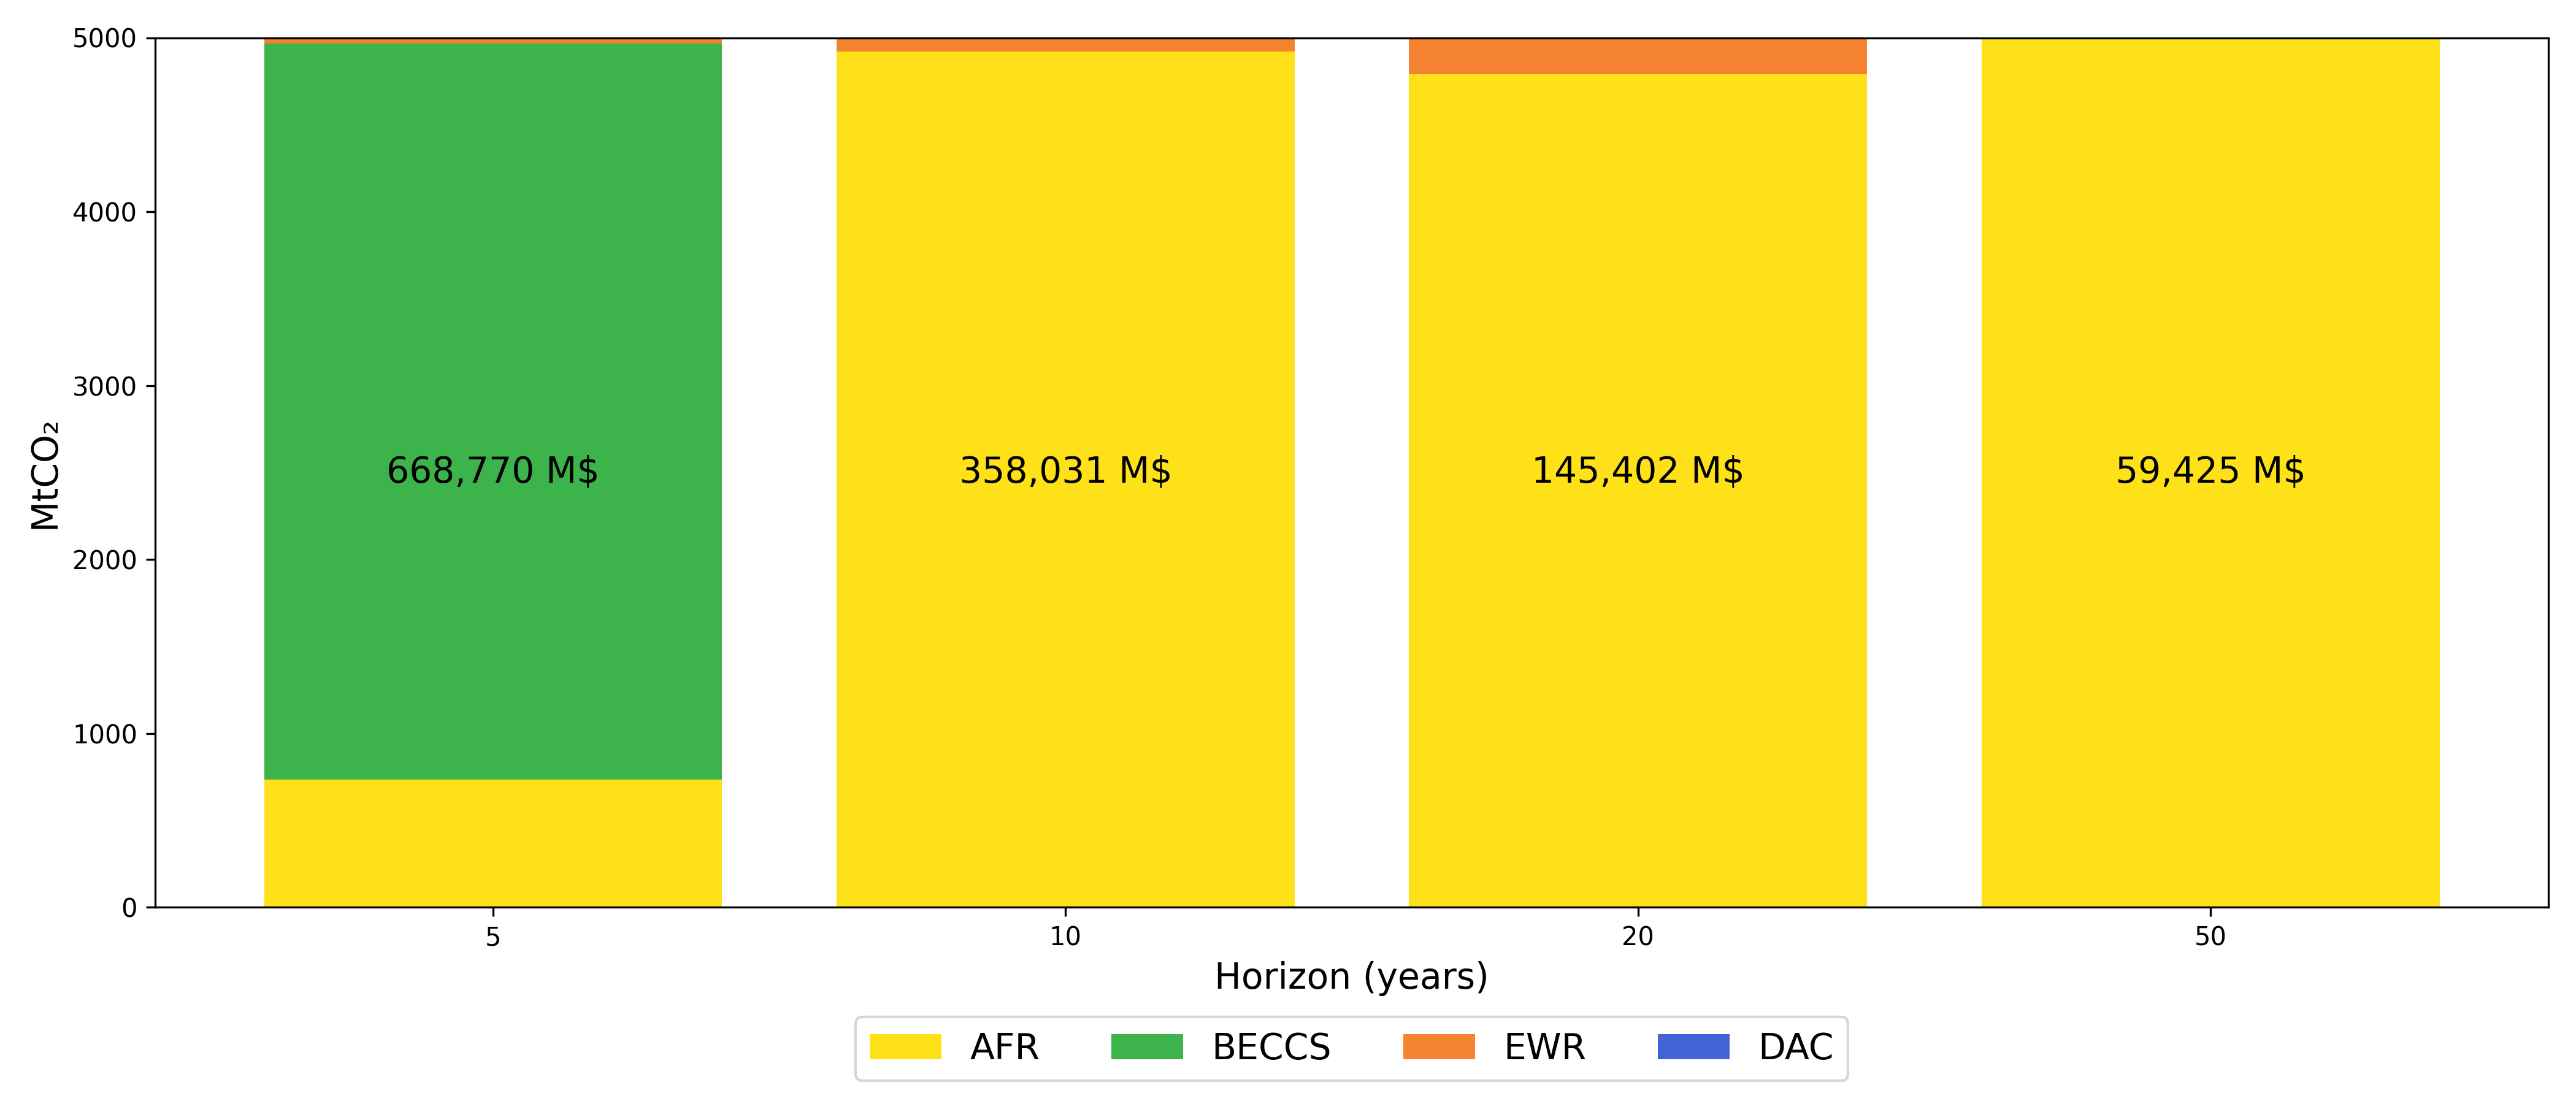
\includegraphics[width=1\linewidth]{figures/overall_static_optimization_bars.png}
    \caption{Optimal static portfolio (5 Gt CDR)}
    \label{fig:overall_static_optimization_bars}
  \end{center}
  \vspace*{-\baselineskip}
\end{figure}

The results of the second model (Fig 4.2) are largely similar, with the notable difference that a larger amount of BECCS CDR is  required even for the longer time horizons, due to the need to fully ramp up the annual removal from the first year. For a comparison of the different NET's contributions over time, see Appendix A.3.\vspace{2mm}

\begin{figure}[ht!]
  \begin{center}
    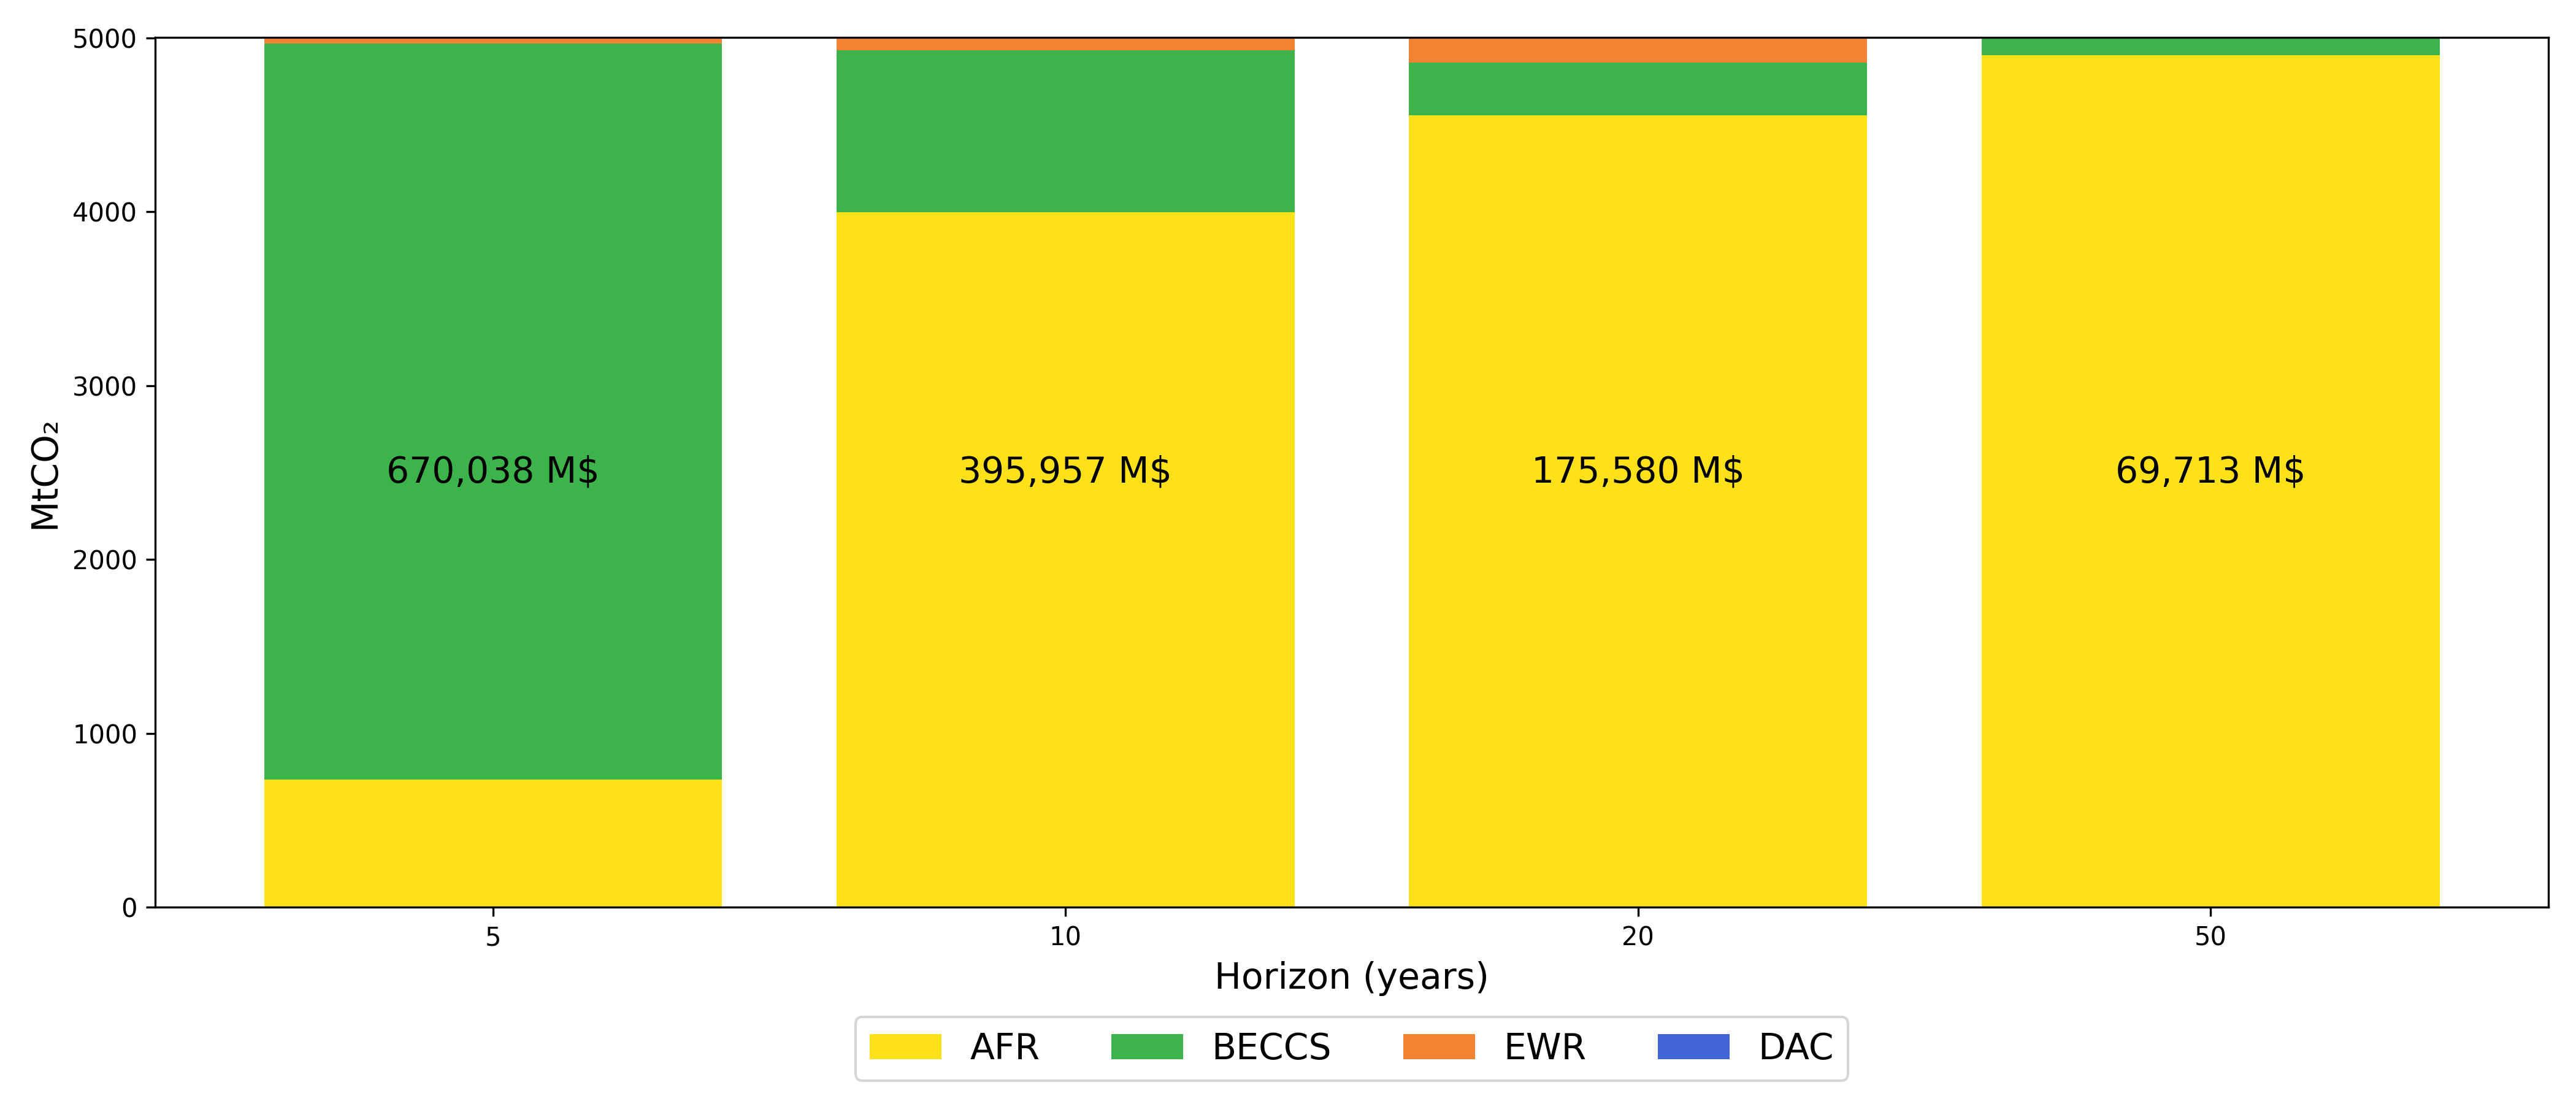
\includegraphics[width=1\linewidth]{figures/annual_static_optimization_bars.png}
    \caption{Optimal static portfolio (5 Gt CDR), equally spread}
    \label{fig:annual_static_optimization_bars}
  \end{center}
  \vspace*{-\baselineskip}
\end{figure}

For both models, the longest time-frame (50 years) is an entire order of magnitude cheaper in overall costs than the shortest time-frame (five years). This is caused partially by the shorter time-frames requiring a larger amount of BECCS in order to quickly achieve the target. Additionally, the longer time-frames allow the afforested trees to grow for longer and take up more CO$_2$, reducing the overall cost further.